%!TEX root = ./template-skripsi.tex
%-------------------------------------------------------------------------------
% 								BAB I
% 							LATAR BELAKANG
%-------------------------------------------------------------------------------

\chapter{PENDAHULUAN}

\section{Latar Belakang Masalah}

Perikanan merupakan suatu sumber penghasilan terbesar yang ada di Indonesia dikarenakan Indonesia sendiri disebut sebagai Negara Maritim yang memiliki arti Negara Kepulauan. Oleh karena itu, banyak penduduk di Indonesia yang bermata pencaharian sebagai petani ikan. Namun, jika terlalu banyak menangkap ikan akan menyebabkan \textit{over fishing} yang membuat kemampuan bereproduksi ikan akan jauh lebih kecil daripada jumlah ikan hasil tangkapan. Hal ini akan menyebabkan langkanya spesies ikan tersebut dan berkurangnya angka produksi ikan. Dengan demikian, untuk mengatasi hal tersebut diperlukan budidaya perikanan yang berguna untuk menjaga ikan sampai masa panen tiba, serta dapat meningkatkan nilai ekonomi para petani ikan.

Dalam menjalankan budidaya perikanan, kebanyakan petani ikan masih melakukan cara manual dalam mengelola budidayanya. Hal ini tentunya kurang efektif dalam jangka panjang dan akan menyulitkan dalam pengelolaan budidayanya. Oleh karena itu, dalam penelitian yang dibuat oleh \citep{fishtalk} dan \citep{haucs} dapat berguna dalam menerapkan budidaya perikanan modern.

Yi-Bing Lin dan timnya membuat \textit{smart aquarium} yang bertujuan untuk meningkatkan kualitas akuarium yang bernama FishTalk. FishTalk memungkinkan sebuah sensor pada akuarium untuk menggerakan aktuator secara real time. Kegunaan dari \textit{smart aquarium} ini seperti sistem pemberian pakan otomatis dan pengendalian air dalam kolam secara otomatis. \citep{fishtalk}

Sementara itu, Bing Ouyang dan timnya membuat sebuah sistem yang dibentuk dan digunakan untuk monitoring serta \textit{decision making} pada tambak perikanan, sistem ini dinamakan HAUCS (\textit{Hybrid Aerial Underwater Robotic System}). Pemantauan ini dilakukan dengan memanfaatkan sistem robotik, mesin, dan operator manusia. Tujuan dibentuknya HAUCS ini adalah untuk meringankan pekerjaan manusia dari tugas yang berat, terlalu banyak biaya, dan memakan waktu dalam operasi pelaksanaan budidaya \textit{aquaculture} melalui platform pemanfaatan sistem robotik. \citep{haucs}

Dari kedua penelitian diatas, dapat disimpulkan bahwa alat yang digunakan dapat bermanfaat bagi para petani ikan karena dapat mempermudah pengelolaan budidaya. Namun, tentunya alat dan bahan yang dibutuhkan cukup banyak dan pasti mematok harga yang tidak sedikit. 

Oleh karena itu, penelitian yang dilakukan oleh \citep{waterquality} dan timnya mungkin dapat mengatasi masalah tersebut. Penelitian ini bertujuan untuk membuat big data dengan framework SpringBoot dan Java Persistence API (JPA) yang didalamnya terdapat data kualitas air pada setiap perkembangbiakan ikan ternak. Platform ini dapat digunakan untuk memprediksi kualitas air dari setiap kolam dan memberikan notifikasi langsung ketika ada masalah pada kolam tersebut. Namun, penelitian ini hanya berfokus pada pendataan kualitas air saja sehingga rincian lain dari budidaya tersebut masih belum lengkap. \citep{waterquality} 

Tapi, tidak seperti dua penelitian yang sudah dirujuk sebelumnya, penelitian \citep{waterquality} ini berbasis aplikasi sehingga tidak ada biaya peralatan tambahan. Dengan demikian, petani ikan akan lebih terbantu jika terdapat aplikasi yang dapat membantu mereka dalam mengembangkan budidayanya tanpa perlu mengeluarkan biaya tambahan.

Pada penelitian yang dilakukan oleh \citep{fadhil2021}, \citep{gian2022} dan \citep{andri2022}, mereka membuat suatu aplikasi yang berfungsi untuk mencatat pendetailan dari setiap budidaya para petani ikan. Detail yang dimaksud seperti pencatatan pakan ikan, pencatatan angka kematian ikan, pengendalian kualitas air, dan pencatatan lainnya yang berhubungan pada musim budidaya ikan tersebut. Aplikasi ini tentunya dapat membantu para petani ikan dan juga dapat meningkatkan ekonomi petani ikan sejalan dengan lancarnya musim budidaya.

Penelitian yang terkait dalam aplikasi tersebut adalah penelitian Fadhil Perwira Hadi yang berjudul “Rancang Bangun Web Service dan Website sebagai Storage Engine dan Monitoring Data Sensing untuk Budidaya Ikan Air Tawar” menghasilkan suatu sistem web service yang dapat menerima data yang dikirimkan oleh embedded device, dengan menerapkan konsep IoT \citep{fadhil2021}. Web service tersebut kemudian dilanjutkan dengan penelitian Andri Rahmanto dengan judul “Perancangan Arsitektur Aplikasi Budidaya Perikanan Modern pada Backend yang bertanggung jawab dalam melayani Transaksi Query Webservice dengan menggunakan Teknologi Flask Microservice”. Web service ini menghasilkan output berupa arsitektur aplikasi budidaya perikanan modern pada backend berupa endpoint yang dapat digunakan untuk pendataan budidaya perikanan air tawar \citep{andri2022}. Dalam pengolahan backend ini, Gian Chiesa Maghriza dengan penelitiannya yang berjudul “Perancangan Frontend Aplikasi Pendukung Teknologi Perikanan Modern dengan menggunakan Framework Flutter yang mentarget Multi Platform” membuat \textit{user interface} serta konfigurasi fitur pencatatan dari aplikasi teknologi perikanan modern. Fitur-fitur yang ada pada aplikasi ini didasari pada penggunaan endpoint yang sudah disediakan pada backend buatan Andri dan juga penelitian ini mentargetkan \textit{multi platform} yang berarti bisa digunakan pada perangkat Android dan iOS \citep{gian2022}. Namun pada aplikasi tersebut masih terdapat kekurangan seperti belum tersedia fitur inventarisasi sebagai \textit{storage} dalam budidaya dan juga aplikasi tersebut masih single user dalam penggunaannya, sehingga para petani hanya dapat menggunakan aplikasi tersebut tanpa adanya koneksi antar petani ikan yang lain.

Hal tersebut tentunya masih belum memecahkan masalah dari petani ikan dalam menjalankan budidayanya. Masalah yang paling berdampak pada petani ikan adalah saat harga komoditas mengalami kenaikan sedangkan harga jual ikan tidak mengalami perubahan dikarenakan harga yang sudah ditetapkan oleh Kemendagri sehingga petani bisa mengalami kerugian. Hal ini tentunya akan membawa dampak negatif dalam nilai ekonomi pertanian perikanan.

Oleh karena itu, penelitian ini bertujuan untuk memecahkan masalah tersebut dengan menambahkan sistem multi user serta inventarisasi pada aplikasi teknologi perikanan modern ini. Tujuan dari ditambahkannya multi user adalah agar aplikasi ini bisa dipakai oleh banyak petani atau lembaga yang bergerak di bidang budidaya ikan air tawar dan pencatatan dari setiap musim budidaya petani atau lembaga perusahaan tersebut akan di publish kedalam aplikasi dan dapat dilihat oleh pembudidaya air tawar yang lain. Dengan demikian, sesama pembudidaya ikan air tawar dapat mengembangkan sistem budidaya perikanan air tawar yang lebih stabil khususnya untuk petani yang mendapatkan profit kecil. 

Sementara itu, fitur inventarisasi akan sangat membantu petani dalam mengolah profit budidayanya karena fitur ini dapat mengontrol kebutuhan dan pengeluaran dalam setiap proses budidaya ikan air tawar sehingga pembudidaya dapat menghitung profit dan dapat mendapatkan detil informasi dari setiap budidaya yang dilakukan.

Berdasarkan fitur baru yang sudah dijelaskan sebelumnya, aplikasi ini diharapkan dapat membantu para petani ikan dalam berbudidaya sehingga petani ikan dapat mendapatkan keuntungan disetiap musim budidayanya.

% \begin{figure}[H]
% 	\centering
% 	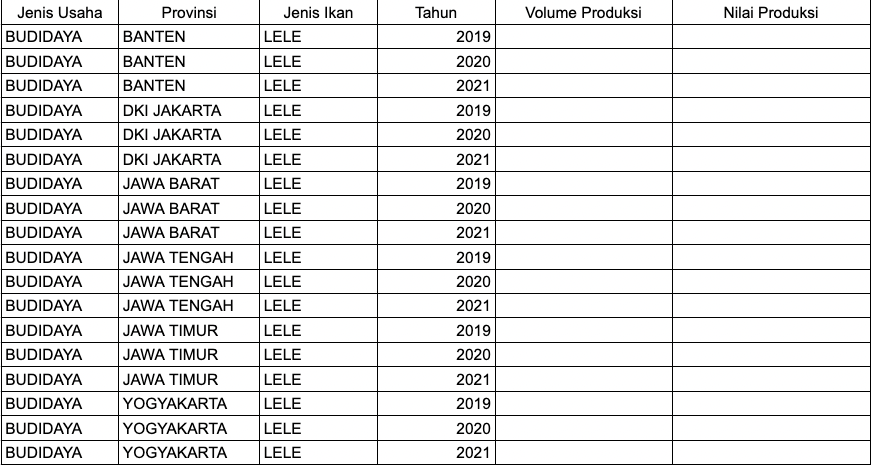
\includegraphics[keepaspectratio, width=12cm]{gambar/budidaya-ikan-lele-jawa.png}
% 	\caption{\emph{Produksi Ikan Lele Di Pulau Jawa} \citep{kkpdatajawa}}
% 	\label{gambar:budidaya-ikan-lele-jawa}
% \end{figure}

\section{Rumusan Masalah}
Dari uraian latar belakang di atas, perumusan masalah pada penelitian ini ialah “Bagaimana perancangan aplikasi yang mendukung \emph{multi user} dan inventarisasi yang menjadi pendukung dalam menjalankan budidaya perikanan modern?”

\section{Pembatasan Masalah}
Pembatasan masalah pada penelitian ini antara lain:
\begin{enumerate}
	\item Aplikasi dikembangkan untuk banyak user.
	\item Pengembangan aplikasi menggunakan \emph{Framework} Flutter.
	\item Pengembangan \emph{web service} menggunakan \emph{Framework} Flask.
\end{enumerate}

\section{Tujuan Penelitian}
	Penelitian ini dilakukan dengan tujuan untuk membuat aplikasi budidaya ikan modern dengan penerapan \emph{multi user} dan inventarisasi berbasis \emph{multi platform}.

\section{Manfaat Penelitian}
\begin{enumerate}
	\item Bagi penulis
		
	Meningkatkan pengetahuan tentang teknologi budidaya perikanan modern, menambah pengalaman dalam mengembangkan aplikasi, memperoleh gelar sarjana di bidang Ilmu Komputer, serta menjadi media untuk penulis dalam mengaplikasikan ilmu yang didapat dari kampus.
		
	\item Bagi Universitas Negeri Jakarta
	 	
	Menjadi pedoman untuk penelitian di masa depan, dan dapat memberikan panduan bagi mahasiswa program studi Ilmu Komputer tentang rancang bangun aplikasi teknologi budidaya perikanan modern.
	
	\item Bagi masyarakat
	 	
	Membantu masyarakat yang ingin dan sedang menggeluti bidang budidaya perikanan dalam proses pendataan ikan dan pengelolaan lingkungan dalam budidaya itu sendiri.
	 			
\end{enumerate}


% Baris ini digunakan untuk membantu dalam melakukan sitasi
% Karena diapit dengan comment, maka baris ini akan diabaikan
% oleh compiler LaTeX.
\begin{comment}
\bibliography{daftar-pustaka}
\end{comment}
